% report.tex

% change pdflatex below to xelatex if you use Chinese
% !TEX program = pdflatex
\documentclass[]{beamer}

\input{preamble}
\input{newcommands}

% Additional packages for this presentation
\usepackage{tikz}
\usetikzlibrary{shapes,arrows,positioning}
\usepackage{listings}
\lstset{
  basicstyle=\ttfamily\small,
  breaklines=true,
  frame=single,
  language=C,
  showstringspaces=false
}

%%%%%%%%%%%%%%%%%%%%%%%%%%%%%%%%%%%%%%%%%%%%%%%%%%%%%%%%%%%%%%%%%%%%%%%%%%%%%%%%
\title[Teaching PL in the LLM Era]{Teaching Programming Languages \\
in the Era of Large Language Models}
\subtitle{\teal{What to Teach, What Not to Teach, and Why}}

\author[Hengfeng Wei]{Hengfeng Wei}
\titlegraphic{
  \includegraphics[height = 1.5cm]{figs/nju-logo-purple}~
  \includegraphics[height = 1.5cm]{figs/software-logo}}
\institute{hfwei@nju.edu.cn}
\date{\today}
%%%%%%%%%%%%%%%%%%%%
\begin{document}
\maketitle
%%%%%%%%%%%%%%%%%%%%
% intro.tex
% Introduction and Outline

%%%%%%%%%%%%%%%%%%%%
\begin{frame}{Outline}
  \tableofcontents
  
  % Speaker note: Mention this is a 20-30 minute presentation
\end{frame}
%%%%%%%%%%%%%%%%%%%%
%%%%%%%%%%%%%%%%%%%%
% motivation.tex
% Section 1: Why Programming Education Must Change in the LLM Era

%%%%%%%%%%%%%%%%%%%%
\section{Motivation: Why Programming Education Must Change}
%%%%%%%%%%%%%%%%%%%%

%%%%%%%%%%%%%%%%%%%%
\begin{frame}{The LLM Revolution in Programming}
  \begin{center}
    \textbf{Large Language Models have fundamentally changed how we write code.}
  \end{center}
  
  \vspace{0.5cm}
  
  \begin{columns}[T]
    \begin{column}{0.48\textwidth}
      \textbf{\teal{What LLMs Excel At:}}
      \begin{itemize}
        \item Syntax generation
        \item API lookups
        \item Boilerplate code
        \item Pattern matching
        \item Documentation retrieval
      \end{itemize}
    \end{column}
    \begin{column}{0.48\textwidth}
      \textbf{\red{What LLMs Struggle With:}}
      \begin{itemize}
        \item Deep semantic reasoning
        \item Undefined behavior analysis
        \item Memory model understanding
        \item Design trade-off evaluation
        \item Historical context
      \end{itemize}
    \end{column}
  \end{columns}
  
  % Speaker note: Emphasize that LLMs shift the bottleneck from syntax recall to conceptual reasoning
\end{frame}
%%%%%%%%%%%%%%%%%%%%

%%%%%%%%%%%%%%%%%%%%
\begin{frame}{The Shifting Bottleneck}
  \begin{center}
    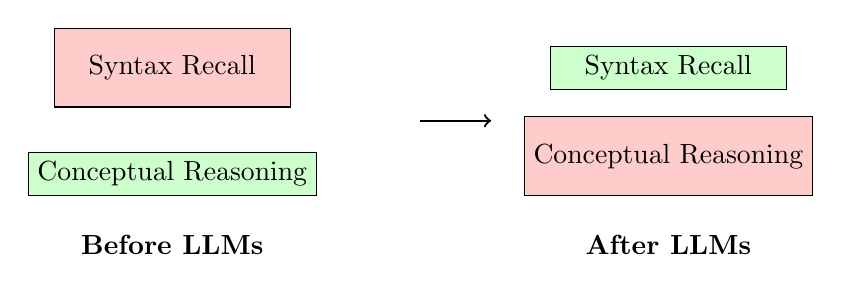
\begin{tikzpicture}[scale=0.9]
      % Before LLMs
      \node[draw, rectangle, fill=red!20, minimum width=3cm, minimum height=1cm] at (-3.5, 2) {Syntax Recall};
      \node[draw, rectangle, fill=green!20, minimum width=3cm, minimum height=0.5cm] at (-3.5, 0.5) {Conceptual Reasoning};
      \node at (-3.5, -0.5) {\textbf{Before LLMs}};
      
      % After LLMs
      \node[draw, rectangle, fill=green!20, minimum width=3cm, minimum height=0.5cm] at (3.5, 2) {Syntax Recall};
      \node[draw, rectangle, fill=red!20, minimum width=3cm, minimum height=1cm] at (3.5, 0.75) {Conceptual Reasoning};
      \node at (3.5, -0.5) {\textbf{After LLMs}};
      
      % Arrow
      \draw[->, thick] (0, 1.25) -- (1, 1.25);
    \end{tikzpicture}
  \end{center}
  
  \vspace{0.3cm}
  
  \begin{block}{Key Insight}
    The bottleneck has shifted from \textbf{remembering syntax} to \textbf{understanding why code works} (or doesn't).
  \end{block}
  
  % Speaker note: Reference Perlis's Epigram #7: "It is easier to write an incorrect program than understand a correct one."
\end{frame}
%%%%%%%%%%%%%%%%%%%%

%%%%%%%%%%%%%%%%%%%%
\begin{frame}[fragile]{The Danger: LLM Hallucinated Correctness}
  \textbf{Example: LLM-generated C code with hidden undefined behavior}
  
  \begin{block}{Seemingly Correct Code}
\begin{verbatim}
int *get_array_element(int *arr, size_t index) {
    return &arr[index];  // No bounds checking!
}

int sum_array(int *a, int *b, int n) {
    int sum = 0;
    for (int i = 0; i < n; i++)
        sum += a[i] + b[i];  // Aliasing issue!
    return sum;
}
\end{verbatim}
  \end{block}
  
  \vspace{0.2cm}
  \red{\textbf{Problems:}} Buffer overflow, pointer aliasing violations (C99 Rationale, \S6.5)
  
  % Speaker note: LLMs generate syntactically correct code that may invoke undefined behavior
\end{frame}
%%%%%%%%%%%%%%%%%%%%

%%%%%%%%%%%%%%%%%%%%
\begin{frame}{Why Understanding Design Rationale Matters}
  \begin{quote}
    ``C is a language that trusts the programmer.'' \\
    \hfill --- \textit{Dennis Ritchie, The Development of the C Language}
  \end{quote}
  
  \vspace{0.5cm}
  
  \textbf{Students must understand:}
  \begin{enumerate}
    \item \textbf{Why} C has undefined behavior (optimization freedom)
    \item \textbf{Why} Java has checked exceptions (explicit error handling)
    \item \textbf{Why} memory alignment exists (hardware constraints)
    \item \textbf{How} design choices affect real-world code
  \end{enumerate}
  
  \vspace{0.3cm}
  
  \begin{alertblock}{Teaching Implication}
    LLMs cannot teach \textit{why}---only instructors can provide historical and philosophical context.
  \end{alertblock}
  
  % Speaker note: Reference "The Development of the C Language" by Ritchie
\end{frame}
%%%%%%%%%%%%%%%%%%%%

%%%%%%%%%%%%%%%%%%%%
\begin{frame}{Execution Model Literacy Remains Critical}
  \begin{columns}[T]
    \begin{column}{0.55\textwidth}
      \textbf{What Students Must Understand:}
      \begin{itemize}
        \item C's abstract machine model
        \item Memory layout (stack, heap, data segments)
        \item Object lifetime and storage duration
        \item Sequence points and side effects
        \item The ``as-if'' rule
      \end{itemize}
    \end{column}
    \begin{column}{0.43\textwidth}
      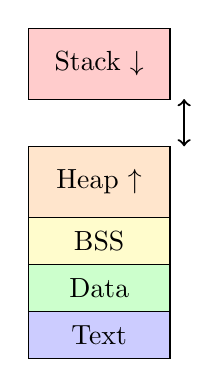
\begin{tikzpicture}[scale=0.6]
        \draw[fill=blue!20] (0,0) rectangle (3,1);
        \node at (1.5,0.5) {Text};
        \draw[fill=green!20] (0,1) rectangle (3,2);
        \node at (1.5,1.5) {Data};
        \draw[fill=yellow!20] (0,2) rectangle (3,3);
        \node at (1.5,2.5) {BSS};
        \draw[fill=orange!20] (0,3) rectangle (3,4.5);
        \node at (1.5,3.75) {Heap $\uparrow$};
        \draw[fill=red!20] (0,5.5) rectangle (3,7);
        \node at (1.5,6.25) {Stack $\downarrow$};
        \draw[<->, thick] (3.3, 4.5) -- (3.3, 5.5);
      \end{tikzpicture}
    \end{column}
  \end{columns}
  
  \vspace{0.3cm}
  
  \begin{block}{Reference: ISO C23 \S5.1.2.3}
    ``The semantic descriptions in this document describe the behavior of an abstract machine...''
  \end{block}
  
  % Speaker note: LLMs cannot reason about execution models without explicit training
\end{frame}
%%%%%%%%%%%%%%%%%%%%

%%%%%%%%%%%%%%%%%%%%
% core-concepts.tex
% Section 2: What Should STILL Be Taught (Core Concepts)

%%%%%%%%%%%%%%%%%%%%
\section{What Should STILL Be Taught}
%%%%%%%%%%%%%%%%%%%%

%%%%%%%%%%%%%%%%%%%%
\begin{frame}{Core Concepts LLMs Cannot Replace}
  \begin{center}
    \textbf{Focus on concepts that require \underline{deep understanding}, not memorization.}
  \end{center}
  
  \vspace{0.3cm}
  
  \begin{enumerate}
    \item \textbf{Historical Development} --- Why languages evolved as they did
    \item \textbf{Design Philosophy} --- Minimalism (C) vs. Safety (Java)
    \item \textbf{Execution \& Memory Models} --- How programs actually run
    \item \textbf{Type Systems \& Runtime Systems} --- Static vs. dynamic guarantees
    \item \textbf{Interface/ABI Stability} --- Binary compatibility constraints
    \item \textbf{Cost Models} --- Compiler transformations, UB, virtual dispatch
  \end{enumerate}
  
  \vspace{0.3cm}
  
  \begin{alertblock}{Principle}
    Teach \textit{understanding} over \textit{recitation}. (cf. Perlis, Epigrams on Programming)
  \end{alertblock}
  
  % Speaker note: These are areas where human expertise provides irreplaceable value
\end{frame}
%%%%%%%%%%%%%%%%%%%%

%%%%%%%%%%%%%%%%%%%%
\begin{frame}{Historical Development of C}
  \begin{columns}[T]
    \begin{column}{0.5\textwidth}
      \textbf{Timeline:}
      \begin{itemize}
        \item 1969--1973: C developed at Bell Labs
        \item 1978: K\&R ``The C Programming Language''
        \item 1989: ANSI C (C89)
        \item 1999: C99 (VLAs, \texttt{restrict}, inline)
        \item 2011: C11 (atomics, threads)
        \item 2023: C23 (modern features)
      \end{itemize}
    \end{column}
    \begin{column}{0.48\textwidth}
      \textbf{Design Philosophy:}
      \begin{quote}
        ``Trust the programmer.'' \\
        ``Keep the language small and simple.'' \\
        ``Make it fast, even if not guaranteed portable.''
      \end{quote}
      \hfill --- \textit{Dennis Ritchie}
    \end{column}
  \end{columns}
  
  \vspace{0.3cm}
  
  \begin{block}{Teaching Point}
    Understanding \textit{why} C was designed this way explains undefined behavior, pointer arithmetic, and the lack of bounds checking.
  \end{block}
  
  % Speaker note: Reference "The Development of the C Language" (Ritchie, 1993)
\end{frame}
%%%%%%%%%%%%%%%%%%%%

%%%%%%%%%%%%%%%%%%%%
\begin{frame}[fragile]{Example 1: Pointer Aliasing and Undefined Behavior}
  \begin{columns}[T]
    \begin{column}{0.48\textwidth}
      \textbf{Strict Aliasing Rule:}
      \begin{block}{UB Example}
\begin{verbatim}
float f = 3.14f;
int *ip = (int *)&f;
int i = *ip;  // UB!
\end{verbatim}
      \end{block}
      
      \begin{block}{Correct Approach}
\begin{verbatim}
float f = 3.14f;
int i;
memcpy(&i, &f, sizeof(i));
\end{verbatim}
      \end{block}
    \end{column}
    \begin{column}{0.48\textwidth}
      \textbf{Why UB Exists:}
      \begin{block}{Signed Overflow}
\begin{verbatim}
int x = INT_MAX;
x = x + 1;  // UB!
\end{verbatim}
      \end{block}
      
      \textbf{Enables:}
      \begin{itemize}
        \item Loop optimizations
        \item Vectorization
        \item Dead code elimination
      \end{itemize}
    \end{column}
  \end{columns}
  
  \vspace{0.2cm}
  
  \begin{alertblock}{C99 Rationale}
    ``Undefined behavior gives the implementor license not to catch certain program errors...''
  \end{alertblock}
  
  % Speaker note: UB is a feature, not a bug---but must be taught carefully
\end{frame}
%%%%%%%%%%%%%%%%%%%%

%%%%%%%%%%%%%%%%%%%%
\begin{frame}[fragile]{Example 2: Memory Layout and Alignment}
  \begin{columns}[T]
    \begin{column}{0.48\textwidth}
      \begin{block}{Struct Definition}
\begin{verbatim}
struct example {
    char a;    // 1 byte
    int  b;    // 4 bytes
    char c;    // 1 byte
};
// sizeof = 12, not 6!
\end{verbatim}
      \end{block}
      
      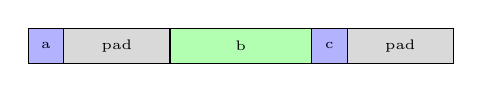
\begin{tikzpicture}[scale=0.45]
        \draw[fill=blue!30] (0,0) rectangle (1,1);
        \node at (0.5,0.5) {\tiny a};
        \draw[fill=gray!30] (1,0) rectangle (4,1);
        \node at (2.5,0.5) {\tiny pad};
        \draw[fill=green!30] (4,0) rectangle (8,1);
        \node at (6,0.5) {\tiny b};
        \draw[fill=blue!30] (8,0) rectangle (9,1);
        \node at (8.5,0.5) {\tiny c};
        \draw[fill=gray!30] (9,0) rectangle (12,1);
        \node at (10.5,0.5) {\tiny pad};
      \end{tikzpicture}
    \end{column}
    \begin{column}{0.48\textwidth}
      \begin{block}{Pointers to Pointers}
\begin{verbatim}
int x = 42;
int *p = &x;
int **pp = &p;
**pp = 100;  // x = 100
\end{verbatim}
      \end{block}
      
      \textbf{Real-World Uses:}
      \begin{itemize}
        \item Dynamic 2D arrays
        \item Linked list insertion
        \item Output parameters
      \end{itemize}
    \end{column}
  \end{columns}
  
  % Speaker note: Real-world impact on network protocols, file formats
\end{frame}
%%%%%%%%%%%%%%%%%%%%

%%%%%%%%%%%%%%%%%%%%
\begin{frame}[fragile]{Example 3: Library Design and Security}
  \textbf{P.J. Plauger's Principles + CERT C Secure Coding}
  
  \begin{columns}[T]
    \begin{column}{0.48\textwidth}
      \begin{block}{\texttt{gets} vs. \texttt{fgets}}
\begin{verbatim}
// DANGEROUS (removed in C11)
gets(buf);

// SAFE
fgets(buf, sizeof(buf), 
      stdin);
\end{verbatim}
      \end{block}
    \end{column}
    \begin{column}{0.48\textwidth}
      \begin{block}{STR31-C: Null termination}
\begin{verbatim}
strncpy(dest, src, 
        sizeof(dest));
dest[sizeof(dest)-1] = '\0';
\end{verbatim}
      \end{block}
    \end{column}
  \end{columns}
  
  \vspace{0.3cm}
  
  \textbf{Design Principles (Plauger):}
  \begin{itemize}
    \item Minimal interface, maximum functionality
    \item Composable primitives (\texttt{fopen}, \texttt{fread}, \texttt{fclose})
    \item Error handling via return values (not exceptions)
  \end{itemize}
  
  \textbf{Teaching Point:} Security vulnerabilities stem from misunderstanding semantics.
  
  % Speaker note: Reference SEI CERT C Coding Standard (2016)
\end{frame}
%%%%%%%%%%%%%%%%%%%%

%%%%%%%%%%%%%%%%%%%%
\begin{frame}[fragile]{Java Examples: Lambdas and GC Trade-offs}
  \begin{columns}[T]
    \begin{column}{0.48\textwidth}
      \textbf{Lambda Implementation:}
      \begin{block}{Source}
\begin{verbatim}
names.forEach(s -> 
    System.out.println(s));
\end{verbatim}
      \end{block}
      
      \textbf{Under the Hood:}
      \begin{itemize}
        \item \texttt{invokedynamic} instruction
        \item \texttt{LambdaMetafactory} generates class
        \item Captured vars become fields
        \item Explains ``effectively final''
      \end{itemize}
    \end{column}
    \begin{column}{0.48\textwidth}
      \textbf{GC vs. Manual Memory:}
      
      \textbf{\teal{Java GC:}}
      \begin{itemize}
        \item No use-after-free/double-free
        \item Simpler programming model
      \end{itemize}
      
      \textbf{\red{Java GC Costs:}}
      \begin{itemize}
        \item Stop-the-world pauses
        \item Memory overhead
        \item Unpredictable latency
      \end{itemize}
    \end{column}
  \end{columns}
  
  \vspace{0.2cm}
  
  \textbf{Teaching Point:} Students must understand \textit{why} both approaches exist.
  
  % Speaker note: Compare with C's malloc/free and C++'s RAII
\end{frame}
%%%%%%%%%%%%%%%%%%%%

%%%%%%%%%%%%%%%%%%%%
% de-emphasize.tex
% Section 3: What Should Be DE-Emphasized

%%%%%%%%%%%%%%%%%%%%
\section{What Should Be DE-Emphasized}
%%%%%%%%%%%%%%%%%%%%

%%%%%%%%%%%%%%%%%%%%
\begin{frame}{Topics to Reduce or Remove}
  \begin{center}
    \textbf{LLMs excel at syntax trivia and mechanical tasks.} \\
    \textit{Stop testing what machines do better.}
  \end{center}
  
  \vspace{0.5cm}
  
  \begin{columns}[T]
    \begin{column}{0.48\textwidth}
      \textbf{\red{De-emphasize:}}
      \begin{itemize}
        \item Syntax corner cases
        \item Operator precedence trivia
        \item Rarely-used features
        \item Mechanical library usage
        \item Boilerplate patterns
        \item Man-page memorization
      \end{itemize}
    \end{column}
    \begin{column}{0.48\textwidth}
      \textbf{\teal{Replace with:}}
      \begin{itemize}
        \item Semantic understanding
        \item Design rationale
        \item Trade-off analysis
        \item Cost model reasoning
        \item Security awareness
        \item Debugging skills
      \end{itemize}
    \end{column}
  \end{columns}
  
  % Speaker note: The goal is to shift from "syntax lawyers" to "language architects"
\end{frame}
%%%%%%%%%%%%%%%%%%%%

%%%%%%%%%%%%%%%%%%%%
\begin{frame}[fragile]{Examples of Outdated Teaching Content}
  \begin{columns}[T]
    \begin{column}{0.48\textwidth}
      \textbf{Precedence Trivia:}
      \begin{block}{Don't Test}
\begin{verbatim}
int y = 3 + x++ * 2;
// What is y?
\end{verbatim}
      \end{block}
      
      \textbf{Better:} ``Why does the Google C++ Style Guide recommend explicit parentheses?''
      
      \vspace{0.3cm}
      
      \textbf{Rare Features:}
      \begin{block}{Trigraphs (C23 removed)}
\begin{verbatim}
??= -> #  // Obsolete
\end{verbatim}
      \end{block}
    \end{column}
    \begin{column}{0.48\textwidth}
      \textbf{API Memorization:}
      
      \textbf{Don't:} ``List all \texttt{strftime()} parameters.''
      
      \textbf{Do:} ``Identify the security vulnerability:''
      \begin{block}{Better Question}
\begin{verbatim}
void log(char *input) {
  char buf[64];
  sprintf(buf, input, ...);
}
// Format string vuln!
\end{verbatim}
      \end{block}
    \end{column}
  \end{columns}
  
  % Speaker note: Focus on understanding, not memorization
\end{frame}
%%%%%%%%%%%%%%%%%%%%

%%%%%%%%%%%%%%%%%%%%
\begin{frame}[fragile]{Low-Value Content and the ``Language Lawyer'' Anti-Pattern}
  \begin{columns}[T]
    \begin{column}{0.48\textwidth}
      \textbf{Don't Waste Time On:}
      
      \textbf{Format specifiers:}
      \begin{itemize}
        \item Don't: ``What's \texttt{\%lld}?''
        \item Do: ``When use inttypes.h?''
      \end{itemize}
      
      \textbf{Type conversions:}
      \begin{itemize}
        \item Don't: ``unsigned + signed = ?''
        \item Do: ``Why is this a security risk?''
      \end{itemize}
      
      \textbf{Implementation details:}
      \begin{itemize}
        \item Don't: ``Size of int on x86-64?''
        \item Do: ``Why implementation-defined?''
      \end{itemize}
    \end{column}
    \begin{column}{0.48\textwidth}
      \begin{alertblock}{Language Lawyer}
        Knows every obscure rule but cannot design or debug real systems.
      \end{alertblock}
      
      \textbf{Signs of Bad Teaching:}
      \begin{itemize}
        \item Exams focus on edge cases
        \item Students memorize, not understand
        \item No real-world connection
      \end{itemize}
      
      \vspace{0.2cm}
      
      \begin{quote}
        \footnotesize
        ``A language that doesn't affect the way you think about programming is not worth knowing.'' --- \textit{Perlis}
      \end{quote}
    \end{column}
  \end{columns}
  
  % Speaker note: Reference Perlis's Epigrams on Programming
\end{frame}
%%%%%%%%%%%%%%%%%%%%

%%%%%%%%%%%%%%%%%%%%
% emphasize-more.tex
% Section 4: What Should Be Emphasized MORE

%%%%%%%%%%%%%%%%%%%%
\section{What Should Be Emphasized MORE}
%%%%%%%%%%%%%%%%%%%%

%%%%%%%%%%%%%%%%%%%%
\begin{frame}{Increase Focus On These Topics}
  \begin{center}
    \textbf{Topics that require human expertise and cannot be outsourced to LLMs.}
  \end{center}
  
  \vspace{0.3cm}
  
  \begin{enumerate}
    \item \textbf{Cost Models} --- How choices affect machine code
    \item \textbf{Compiler Transformations} --- Alias analysis, constant folding, UB exploitation
    \item \textbf{API and Library Design} --- Interface stability, composability
    \item \textbf{Trade-off Reasoning} --- Simplicity vs. power vs. safety
    \item \textbf{Execution Models} --- Translation units, linkage, lifetime
    \item \textbf{Standards Rationale} --- Understanding \textit{why} C23 evolved
  \end{enumerate}
  
  \vspace{0.3cm}
  
  \begin{block}{Key Insight}
    These topics connect code to architecture, history, and engineering judgment.
  \end{block}
  
  % Speaker note: These are areas where experience and deep knowledge matter most
\end{frame}
%%%%%%%%%%%%%%%%%%%%

%%%%%%%%%%%%%%%%%%%%
\begin{frame}[fragile]{Cost Models: \texttt{restrict} and Virtual Dispatch}
  \begin{columns}[T]
    \begin{column}{0.48\textwidth}
      \textbf{The \texttt{restrict} Keyword:}
      \begin{block}{Without \texttt{restrict}}
\begin{verbatim}
void add(int *a, int *b,
         int *c, int n) {
  for (int i = 0; i < n; i++)
    c[i] = a[i] + b[i];
}
// Cannot vectorize
\end{verbatim}
      \end{block}
      With \texttt{restrict}: Compiler \textbf{can} vectorize!
    \end{column}
    \begin{column}{0.48\textwidth}
      \textbf{Virtual Dispatch Cost:}
      \begin{block}{Direct vs. Indirect}
\begin{verbatim}
// C: Direct call
handler(d);  // Inlinable

// Java: vtable lookup
h.handle();  // Indirect
\end{verbatim}
      \end{block}
      
      \textbf{Virtual dispatch:} Load vtable pointer, indirect call, harder to inline.
    \end{column}
  \end{columns}
  
  \vspace{0.3cm}
  
  \textbf{Teaching Point:} Students should understand \textit{when} abstraction costs matter.
  
  % Speaker note: Connect to JIT compilation in Java for optimization
\end{frame}
%%%%%%%%%%%%%%%%%%%%

%%%%%%%%%%%%%%%%%%%%
\begin{frame}[fragile]{Cost Models: Cache-Aware Data Layout}
  \textbf{Data-Oriented Design in C}
  
  \begin{columns}[T]
    \begin{column}{0.48\textwidth}
      \begin{block}{Array of Structs (AoS)}
\begin{verbatim}
struct Entity {
  float x, y, z;    // pos
  float vx, vy, vz; // vel
  float mass;
};
Entity entities[1000];
\end{verbatim}
      \end{block}
      \textbf{Problem:} Cache misses when accessing only positions.
    \end{column}
    \begin{column}{0.48\textwidth}
      \begin{block}{Struct of Arrays (SoA)}
\begin{verbatim}
struct Entities {
  float x[1000];
  float y[1000];
  float z[1000];
  float vx[1000];
  // ...
};
\end{verbatim}
      \end{block}
      \textbf{Benefit:} Better cache utilization for position-only access.
    \end{column}
  \end{columns}
  
  % Speaker note: Essential for game development, scientific computing
\end{frame}
%%%%%%%%%%%%%%%%%%%%

%%%%%%%%%%%%%%%%%%%%
\begin{frame}[fragile]{Compiler Transformations: UB Exploitation}
  \textbf{How Compilers Use Undefined Behavior}
  
  \begin{block}{Example: Null Pointer Check Elimination}
\begin{verbatim}
int *p = get_pointer();
int x = *p;           // Dereference before check
if (p == NULL) {      // Compiler removes this!
    handle_error();   // Dead code
}
\end{verbatim}
  \end{block}
  
  \textbf{Compiler Reasoning:}
  \begin{enumerate}
    \item \texttt{*p} dereferences \texttt{p}
    \item If \texttt{p} were \texttt{NULL}, that would be UB
    \item Program assumes no UB $\Rightarrow$ \texttt{p} cannot be \texttt{NULL}
    \item Therefore, remove the entire \texttt{if} block
  \end{enumerate}
  
  \begin{alertblock}{Teaching Point}
    UB is not ``ignored''---it enables aggressive optimization. Real CVEs result from this!
  \end{alertblock}
  
  % Speaker note: Real CVEs have resulted from this optimization pattern
\end{frame}
%%%%%%%%%%%%%%%%%%%%

%%%%%%%%%%%%%%%%%%%%
\begin{frame}[fragile]{API Design and Execution Models}
  \begin{columns}[T]
    \begin{column}{0.48\textwidth}
      \textbf{POSIX File API Principles:}
      \begin{block}{Example}
\begin{verbatim}
int fd = open("f.txt",
              O_RDONLY);
read(fd, buf, sz);
close(fd);
\end{verbatim}
      \end{block}
      
      \textbf{Design Principles:}
      \begin{itemize}
        \item Handle-based resources
        \item Uniform error signaling
        \item Composability (pipes)
        \item Minimal interface
      \end{itemize}
    \end{column}
    \begin{column}{0.48\textwidth}
      \textbf{Translation Units \& Linkage:}
      \begin{block}{file1.c \& file2.c}
\begin{verbatim}
static int count = 0;
void increment(void) {
  count++;
}
// Both "count" are separate!
\end{verbatim}
      \end{block}
      
      \textbf{Key Concepts:}
      \begin{itemize}
        \item \texttt{static} = internal linkage
        \item No \texttt{static} = external linkage
        \item Linker resolves symbols
      \end{itemize}
    \end{column}
  \end{columns}
  
  % Speaker note: Essential for understanding large C projects like Linux
\end{frame}
%%%%%%%%%%%%%%%%%%%%

%%%%%%%%%%%%%%%%%%%%
\begin{frame}{Trade-offs and Standards Evolution}
  \begin{columns}[T]
    \begin{column}{0.48\textwidth}
      \textbf{Safety vs. Performance:}
      \begin{center}
        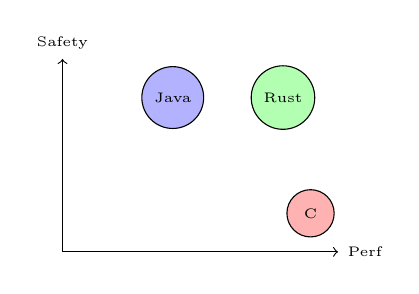
\begin{tikzpicture}[scale=0.7]
          \draw[->] (0,0) -- (5,0) node[right] {\tiny Perf};
          \draw[->] (0,0) -- (0,3.5) node[above] {\tiny Safety};
          \node[draw, circle, fill=red!30, minimum size=0.6cm] at (4.5,0.7) {\tiny C};
          \node[draw, circle, fill=blue!30, minimum size=0.6cm] at (2,2.8) {\tiny Java};
          \node[draw, circle, fill=green!30, minimum size=0.6cm] at (4,2.8) {\tiny Rust};
        \end{tikzpicture}
      \end{center}
      
      Every language makes trade-offs. Students must understand \textit{which} and \textit{why}.
    \end{column}
    \begin{column}{0.48\textwidth}
      \textbf{Why C23 Matters:}
      
      \textbf{Key Changes:}
      \begin{itemize}
        \item \texttt{nullptr} keyword
        \item \texttt{typeof} operator
        \item \texttt{\#embed} directive
        \item Removal of K\&R decls
      \end{itemize}
      
      \textbf{Why?}
      \begin{itemize}
        \item Type safety
        \item Security hardening
        \item C++ compatibility
      \end{itemize}
    \end{column}
  \end{columns}
  
  \vspace{0.2cm}
  
  \textbf{Reference:} ACM Queue ``Catch-23: The New C Standard'' (2023)
  
  % Speaker note: Standards evolution reflects lessons learned
\end{frame}
%%%%%%%%%%%%%%%%%%%%

%%%%%%%%%%%%%%%%%%%%
% case-studies.tex
% Section 5: Pedagogical Case Studies

%%%%%%%%%%%%%%%%%%%%
\section{Pedagogical Case Studies}
%%%%%%%%%%%%%%%%%%%%

%%%%%%%%%%%%%%%%%%%%
\begin{frame}{Case Study Overview}
  \begin{center}
    \textbf{Deep-Dive Examples for Teaching Conceptual Understanding}
  \end{center}
  
  \vspace{0.5cm}
  
  \begin{enumerate}
    \item \textbf{Why C Has Undefined Behavior} --- History + Optimization Rationale
    \item \textbf{How \texttt{malloc}/\texttt{free} Work} --- Fragmentation vs. Speed
    \item \textbf{Java Lambda Desugaring} --- \texttt{invokedynamic} Mechanism
    \item \textbf{C Standard Library Design} --- 1970s Constraints
    \item \textbf{VLA Deprecation \& Large Projects} --- Security + Organization
  \end{enumerate}
  
  \vspace{0.3cm}
  
  \begin{block}{Pedagogical Goal}
    Each case study connects \textit{history} $\rightarrow$ \textit{rationale} $\rightarrow$ \textit{modern practice}.
  \end{block}
  
  % Speaker note: These case studies form the core of deep understanding
\end{frame}
%%%%%%%%%%%%%%%%%%%%

%%%%%%%%%%%%%%%%%%%%
\begin{frame}[fragile]{Case Study 1: Why C Has Undefined Behavior}
  \textbf{Historical Context (Dennis Ritchie, 1993)}
  
  \begin{quote}
    ``C is quirky, flawed, and an enormous success.''
  \end{quote}
  
  \begin{columns}[T]
    \begin{column}{0.48\textwidth}
      \textbf{Origins of UB:}
      \begin{itemize}
        \item \textbf{Portability} --- Ran on diverse hardware
        \item \textbf{Performance} --- No mandatory checks
        \item \textbf{Freedom} --- Compiler knows best
      \end{itemize}
    \end{column}
    \begin{column}{0.48\textwidth}
      \textbf{C99 Rationale Categories:}
      \begin{itemize}
        \item \textbf{Undefined} --- Anything can happen
        \item \textbf{Unspecified} --- Choice not documented
        \item \textbf{Implementation-defined} --- Documented choice
      \end{itemize}
    \end{column}
  \end{columns}
  
  \vspace{0.2cm}
  
  \begin{block}{Compiler Optimization via UB}
\begin{verbatim}
int x = *p;
if (p == NULL) { ... }  // Compiler removes this!
\end{verbatim}
    \textit{After dereferencing, p cannot be NULL (or UB already occurred).}
  \end{block}
  
  % Speaker note: Reference C99 Rationale document Section 4
\end{frame}
%%%%%%%%%%%%%%%%%%%%

%%%%%%%%%%%%%%%%%%%%
\begin{frame}[fragile]{Case Study 2: How \texttt{malloc}/\texttt{free} Work}
  \textbf{Memory Allocator Design Trade-offs}
  
  \begin{columns}[T]
    \begin{column}{0.48\textwidth}
      \begin{center}
        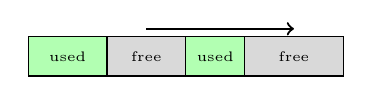
\begin{tikzpicture}[scale=0.5]
          \draw[fill=green!30] (0,0) rectangle (2,1);
          \node at (1,0.5) {\tiny used};
          \draw[fill=gray!30] (2,0) rectangle (4,1);
          \node at (3,0.5) {\tiny free};
          \draw[fill=green!30] (4,0) rectangle (5.5,1);
          \node at (4.75,0.5) {\tiny used};
          \draw[fill=gray!30] (5.5,0) rectangle (8,1);
          \node at (6.75,0.5) {\tiny free};
          \draw[->, thick] (3, 1.2) -- (6.75, 1.2);
        \end{tikzpicture}
      \end{center}
      
      \textbf{Strategies:} First-fit, Best-fit, Buddy system, Slab allocator
    \end{column}
    \begin{column}{0.48\textwidth}
      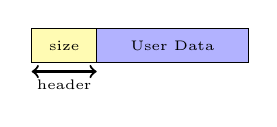
\begin{tikzpicture}[scale=0.55]
        \draw[fill=yellow!30] (0,0) rectangle (1.5,0.8);
        \node at (0.75,0.4) {\tiny size};
        \draw[fill=blue!30] (1.5,0) rectangle (5,0.8);
        \node at (3.25,0.4) {\tiny User Data};
        \draw[<->, thick] (0, -0.2) -- (1.5, -0.2);
        \node at (0.75, -0.5) {\tiny header};
      \end{tikzpicture}
      
      \textbf{Security:} Corrupting metadata enables exploits!
    \end{column}
  \end{columns}
  
  \vspace{0.3cm}
  
  \begin{block}{glibc Implementation}
    Uses bins for different sizes, thread-local caches, and \texttt{mmap} for large allocations. Understanding internals explains buffer overflow vulnerabilities.
  \end{block}
  
  % Speaker note: Reference glibc manual; connect to Java GC trade-offs
\end{frame}
%%%%%%%%%%%%%%%%%%%%

%%%%%%%%%%%%%%%%%%%%
\begin{frame}[fragile]{Case Study 3: Java Lambda Desugaring}
  \textbf{From Source to Bytecode}
  
  \begin{columns}[T]
    \begin{column}{0.48\textwidth}
      \begin{block}{Source Code}
\begin{verbatim}
int mult = 2;
IntUnaryOperator op =
    x -> x * mult;
\end{verbatim}
      \end{block}
      
      \textbf{What JVM Does:}
      \begin{itemize}
        \item \texttt{invokedynamic} instruction
        \item \texttt{LambdaMetafactory} creates class
        \item Captured vars become fields
      \end{itemize}
    \end{column}
    \begin{column}{0.48\textwidth}
      \begin{block}{Equivalent Class}
\begin{verbatim}
class Lambda$$1 {
  final int mult;
  int apply(int x) {
    return x * mult;
  }
}
\end{verbatim}
      \end{block}
      
      \textbf{Benefits:} No class file overhead, JVM can inline, explains ``effectively final'' requirement.
    \end{column}
  \end{columns}
  
  % Speaker note: Explains why captured variables must be effectively final
\end{frame}
%%%%%%%%%%%%%%%%%%%%

%%%%%%%%%%%%%%%%%%%%
\begin{frame}{Case Study 4: C Standard Library Design}
  \textbf{1970s Constraints That Shaped the Library}
  
  \begin{columns}[T]
    \begin{column}{0.48\textwidth}
      \textbf{Hardware Constraints:}
      \begin{itemize}
        \item Limited memory (64KB typical)
        \item Slow I/O devices
        \item No memory protection
        \item Diverse architectures
      \end{itemize}
    \end{column}
    \begin{column}{0.48\textwidth}
      \textbf{Design Decisions:}
      \begin{itemize}
        \item Buffered I/O (\texttt{FILE *})
        \item No bounds checking
        \item Caller allocates buffers
        \item Error codes, not exceptions
      \end{itemize}
    \end{column}
  \end{columns}
  
  \vspace{0.3cm}
  
  \begin{block}{P.J. Plauger, ``The Standard C Library''}
    ``Each function aims to do one thing well, with minimal overhead.''
  \end{block}
  
  \textbf{Teaching Point:} Understanding constraints explains why \texttt{gets()} existed.
  
  % Speaker note: Reference Plauger's book for detailed design rationale
\end{frame}
%%%%%%%%%%%%%%%%%%%%

%%%%%%%%%%%%%%%%%%%%
\begin{frame}[fragile]{Case Study 5: VLA Deprecation \& Large Project Structure}
  \begin{columns}[T]
    \begin{column}{0.48\textwidth}
      \textbf{Why VLA Is Deprecated:}
      \begin{block}{VLA Example (C99)}
\begin{verbatim}
void process(int n) {
  int buffer[n]; // UB risk!
}
\end{verbatim}
      \end{block}
      
      \textbf{Problems:}
      \begin{itemize}
        \item Stack overflow (no bounds check)
        \item Security vulnerability
        \item C11 made optional
        \item CERT C forbids (ARR32-C)
      \end{itemize}
    \end{column}
    \begin{column}{0.48\textwidth}
      \textbf{Linux Kernel Style:}
\begin{verbatim}
- Tabs (8 spaces)
- 80 char lines
- No typedef for structs
- goto for cleanup
\end{verbatim}
      
      \textbf{Why?} Thousands of contributors need consistency, maintainability over cleverness.
    \end{column}
  \end{columns}
  
  \vspace{0.2cm}
  
  \textbf{Teaching Point:} Style guides exist for engineering reasons, not aesthetics.
  
  % Speaker note: Reference Google C++ Style Guide, Professional CMake
\end{frame}
%%%%%%%%%%%%%%%%%%%%

%%%%%%%%%%%%%%%%%%%%
% llm-integration.tex
% Section 6: How to Integrate LLMs in the Curriculum

%%%%%%%%%%%%%%%%%%%%
\section{Integrating LLMs in the Curriculum}
%%%%%%%%%%%%%%%%%%%%

%%%%%%%%%%%%%%%%%%%%
\begin{frame}{Responsible LLM Integration}
  \begin{center}
    \textbf{LLMs are tools, not replacements for learning.}
  \end{center}
  
  \vspace{0.3cm}
  
  \begin{columns}[T]
    \begin{column}{0.48\textwidth}
      \textbf{\teal{Effective Uses:}}
      \begin{itemize}
        \item Code explanation
        \item Debugging assistance
        \item Example generation
        \item Documentation lookup
        \item Boilerplate generation
      \end{itemize}
    \end{column}
    \begin{column}{0.48\textwidth}
      \textbf{\red{Risky Uses:}}
      \begin{itemize}
        \item Blind copy-paste
        \item Security-critical code
        \item Undefined behavior analysis
        \item Performance optimization
        \item Architecture decisions
      \end{itemize}
    \end{column}
  \end{columns}
  
  \vspace{0.3cm}
  
  \begin{block}{Key Principle}
    Teach students to \textit{verify} LLM output, not \textit{trust} it blindly.
  \end{block}
  
  % Speaker note: Students must develop critical evaluation skills
\end{frame}
%%%%%%%%%%%%%%%%%%%%

%%%%%%%%%%%%%%%%%%%%
\begin{frame}[fragile]{LLM-Based Debugging and Code Review}
  \begin{columns}[T]
    \begin{column}{0.48\textwidth}
      \textbf{Debugging Exercise:}
      \begin{block}{Student Code with Bug}
\begin{verbatim}
int *create_array(int n) {
  int arr[n];
  for (int i = 0; i < n; i++)
    arr[i] = i;
  return arr;  // UB!
}
\end{verbatim}
      \end{block}
      
      Ask LLM: ``What's wrong?'' \\
      Then: ``\textit{Why} is this UB?'' \\
      Verify against C standard.
    \end{column}
    \begin{column}{0.48\textwidth}
      \textbf{Code Review Workflow:}
      \begin{enumerate}
        \item Student writes code
        \item Ask LLM for feedback
        \item Critically evaluate suggestions
        \item Instructor verifies
      \end{enumerate}
      
      \textbf{Good Prompts:}
      \begin{itemize}
        \item ``Are there memory leaks?''
        \item ``Is this thread-safe?''
        \item ``Which C rule applies?''
      \end{itemize}
    \end{column}
  \end{columns}
  
  \textbf{Goal:} Use LLMs as starting points, not answers.
  
  % Speaker note: LLMs are good at pattern matching known bugs
\end{frame}
%%%%%%%%%%%%%%%%%%%%

%%%%%%%%%%%%%%%%%%%%
\begin{frame}{Assignment and Exam Design for the LLM Era}
  \begin{columns}[T]
    \begin{column}{0.48\textwidth}
      \textbf{\red{Outdated Assignments:}}
      \begin{itemize}
        \item ``Implement linked list''
        \item ``Write a sorting algorithm''
        \item ``Create a file reader''
      \end{itemize}
      
      \textit{LLMs generate these trivially.}
      
      \vspace{0.3cm}
      
      \textbf{\teal{Modern Assignments:}}
      \begin{itemize}
        \item ``Explain why this has UB''
        \item ``Optimize and measure''
        \item ``Design an API''
        \item ``Review LLM-generated code''
      \end{itemize}
    \end{column}
    \begin{column}{0.48\textwidth}
      \textbf{Exam Questions:}
      
      \textbf{Semantics:}
      \begin{itemize}
        \item ``What memory layout?''
        \item ``Why strict aliasing violation?''
      \end{itemize}
      
      \textbf{Cost Models:}
      \begin{itemize}
        \item ``Which is faster and why?''
        \item ``What does \texttt{restrict} enable?''
      \end{itemize}
      
      \textbf{Design Philosophy:}
      \begin{itemize}
        \item ``Why UB for signed overflow?''
        \item ``Compare C \texttt{errno} vs. Java exceptions''
      \end{itemize}
    \end{column}
  \end{columns}
  
  % Speaker note: Test understanding, not memorization
\end{frame}
%%%%%%%%%%%%%%%%%%%%

%%%%%%%%%%%%%%%%%%%%
\begin{frame}{Classroom LLM Policies and Future}
  \begin{columns}[T]
    \begin{column}{0.48\textwidth}
      \textbf{Clear Guidelines:}
      \begin{enumerate}
        \item \textbf{Disclosure} --- Cite LLM usage
        \item \textbf{Verification} --- No unverified code
        \item \textbf{Understanding} --- Explain all code
        \item \textbf{Attribution} --- Treat as source
      \end{enumerate}
      
      \vspace{0.3cm}
      
      \begin{block}{Sample Policy}
        ``LLMs allowed for learning. All code must be verified, understood, disclosed.''
      \end{block}
    \end{column}
    \begin{column}{0.48\textwidth}
      \textbf{The Future:}
      \begin{center}
        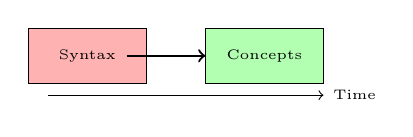
\begin{tikzpicture}[scale=0.5]
          \draw[->] (0,0) -- (7,0) node[right] {\tiny Time};
          \node[draw, rectangle, fill=red!30, minimum width=1.5cm, minimum height=0.7cm, font=\tiny] at (1, 1) {Syntax};
          \node[draw, rectangle, fill=green!30, minimum width=1.5cm, minimum height=0.7cm, font=\tiny] at (5.5, 1) {Concepts};
          \draw[->, thick] (2, 1) -- (4, 1);
        \end{tikzpicture}
      \end{center}
      
      \textbf{What Remains Constant:}
      \begin{itemize}
        \item Execution models
        \item Trade-off reasoning
        \item Debugging skills
        \item API design
      \end{itemize}
    \end{column}
  \end{columns}
  
  \textbf{Key Insight:} Banning LLMs is futile; teaching responsible use is essential.
  
  % Speaker note: Human expertise becomes MORE valuable, not less
\end{frame}
%%%%%%%%%%%%%%%%%%%%

%%%%%%%%%%%%%%%%%%%%
% conclusion.tex
% Section 7: Conclusion

%%%%%%%%%%%%%%%%%%%%
\section{Conclusion}
%%%%%%%%%%%%%%%%%%%%

%%%%%%%%%%%%%%%%%%%%
\begin{frame}{Key Takeaways and Summary}
  \begin{columns}[T]
    \begin{column}{0.48\textwidth}
      \textbf{Teaching Principles:}
      \begin{enumerate}
        \item Shift focus from syntax to semantics
        \item Emphasize history and design rationale
        \item Teach execution and memory models
        \item Use LLMs as tools, not answers
        \item Design assessments for reasoning
      \end{enumerate}
      
      \vspace{0.3cm}
      
      \textbf{\teal{Keep Teaching:}}
      \begin{itemize}
        \item Historical development
        \item Design philosophy
        \item Execution/memory models
        \item Cost models \& security
      \end{itemize}
    \end{column}
    \begin{column}{0.48\textwidth}
      \textbf{\red{De-emphasize:}}
      \begin{itemize}
        \item Syntax trivia
        \item Precedence rules
        \item API memorization
        \item ``Gotcha'' questions
        \item Language lawyering
      \end{itemize}
      
      \vspace{0.3cm}
      
      \begin{block}{Guiding Principle}
        Teach what LLMs \textit{cannot} do: deep reasoning, historical context, design judgment.
      \end{block}
    \end{column}
  \end{columns}
  
  % Speaker note: These principles apply across languages and domains
\end{frame}
%%%%%%%%%%%%%%%%%%%%

%%%%%%%%%%%%%%%%%%%%
\begin{frame}{References and Final Thoughts}
  \begin{columns}[T]
    \begin{column}{0.48\textwidth}
      \textbf{Key References:}
      \begin{itemize}
        \item Ritchie, ``The Development of the C Language'' (1993)
        \item K\&R, ``The C Programming Language'' (1988)
        \item Plauger, ``The Standard C Library'' (1992)
        \item ISO/IEC 9899:2023 (C23)
        \item C99 Rationale (V5.10)
        \item SEI CERT C Coding Standard
        \item ACM Queue ``Catch-23'' (2023)
        \item Perlis, ``Epigrams on Programming''
      \end{itemize}
    \end{column}
    \begin{column}{0.48\textwidth}
      \begin{center}
        \begin{quote}
          ``A language that doesn't affect the way you think about programming is not worth knowing.''
          
          \hfill --- \textit{Perlis, Epigram \#19}
        \end{quote}
        
        \vspace{0.5cm}
        
        \textbf{Our goal:} \\
        Train students who \underline{think}, \\
        not students who \underline{memorize}.
        
        \vspace{0.3cm}
        
        \textit{LLMs make this more important---and more achievable---than ever.}
      \end{center}
    \end{column}
  \end{columns}
  
  % Speaker note: End with inspiration and call to action
\end{frame}
%%%%%%%%%%%%%%%%%%%%
%%%%%%%%%%%%%%%%%%%%
\thankyou{}
%%%%%%%%%%%%%%%%%%%%
% cite references using \ncite{} and compile with biber
% \begin{frame}[allowframebreaks]
%   \printbibliography
% \end{frame}
%%%%%%%%%%%%%%%%%%%%
% \appendix

\end{document}
%%%%%%%%%%%%%%%%%%%%